This lecture introduces more manifold learning algorithms including
Isomap, LLE, LE, MVU and briefly mentions an analog of JL-lemma in the
manifold setting. 

\section{Non-Linear Dimensionality Reduction}
So far, we've been trying to minimize $||X-UV||_F^2$ with  $U\in \mathbb{R}^{D\times d}$ and $V\in \mathbb{R}^{d\times n}$. In this case, $U$ is modeling a linear combination. But if we have $X=f(V)$ instead, where $f$ is a non-linear, smooth function, then we have a non-linear combination. \\
For example, consider a robot moving its head with angle $\theta$. The image at each angle would be a vector in $\R^{100 \times 100}$. Then, in this case we can learn a mapping from $\theta$ to a vector in $\R^{100 \times 100}$. $\theta$ would be the low-dim representation in this case.\\

\textbf{Idea}: Underlying data follows some kind of manifold. \\

\textbf{Manifold} is a set of points which locally resembles Euclidean space. Specifically, manifold is a topological space such that for each point on manifold, the local neighborhood is homeomorphic to Euclidean space. \textbf{Homeomorphic} means that there exists a continuous bijection that maps from the local neighborhood to the Euclidean space. \\

Agenda for today:
\begin{itemize}
\item Isomap (Isometric mapping)
\item LLE (Locally Linear Embedding)
\item LE (Laplacian Eigenmaps)
\item MVU (Maximum Variance Unfolding)
\item kernel PCA
\item Some open problems and approaches to solve these problems
\end{itemize}

\subsection{Isomap}
\subsubsection*{Goal}
To represent large dimensional data in low dimension, such that global geometry of the manifold is preserved. Applications: computer vision. \\
Question: What is global geometry? The geodesic distances between data points. 

\subsubsection*{Notation}
Input data is $X \in \mathbb{R}^{D\times n}$. Output data $Y \in
\mathbb{R}^{d\times n}$ where $d\ll D$. 

\subsubsection*{How?}
\begin{itemize}
\item Approximate the geodesic distances by computing the shortest
  path on a $k$-nearest neighbor ($k$-NN) graph constructed on the input data
  (note that the $k$-NN graph needs to be connected). Use ASSP (All Source Shortest Path algorithm) to compute the shortest paths.
\item Construct a ``distance" matrix $D^{(G)}_{n\times n}$.
\item Run (classical/metric) MDS (multidimensional scaling) on $D^{(G)}_{n\times n}$ to find
  the corresponding low dimension embedding of $X$ ($\min_{Y} \sum_{i<j}||y_i - y_j|| -
  D^{(G)}_{ij}$). 
  
 \item The number of sample points is usually $O(Vk^d)$ where $V$ is volume and $k,d$ are curvature and intrisic dim respectively. 
\end{itemize}

\begin{figure}
\centering
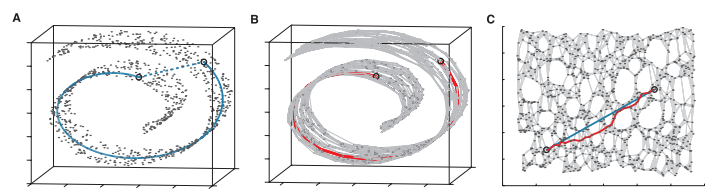
\includegraphics[width=0.7\textwidth]{chapter_7/files/isomap.png}
\caption{Illustration of geodesic distance}
\end{figure}


\subsubsection*{Observations}
\begin{itemize}
\item How well can $k$-NN graph approximate the geodesics.
  \begin{itemize}
  \item Under suitable distributions over the underlying    manifold,
    as $r\rightarrow 0$, $n\rightarrow \infty$, $nr \rightarrow
    \infty$, we can show that ASSP approximates the geodesics. 
  \end{itemize}
 
\begin{figure}
\centering
\begin{tikzpicture}
\draw (2,2) circle (1.5cm);
\draw (10,2) arc[x radius=1.5, y radius=1.5, start angle=0, end angle=-350];
\end{tikzpicture}
\caption{A circle (manifold), as shown on the left, cannot be properly mapped to $\mathbb{R}^{1}$. But if we have a hole, as shown on the right, then it can be embedded to $\mathbb{R}^{1}$. } \label{fig:M1}
\end{figure}
 
\item For what kinds of manifolds does Isomap work? When can geodesic paths become Euclidean paths?
  \begin{itemize}
  \item Underlying manifold needs to be (globally) isometric to some Euclidean space 
    $\mathbb{R}^n$; that is, it has no intrinsic curvature. For
    example, a spherical cap (a hemisphere) cannot be embedded into
    Euclidean space without distorting distances (imagine trying to
    flatten the northern hemisphere of a globe without
    stretching/ripping the map).  
    
\begin{figure}
\centering
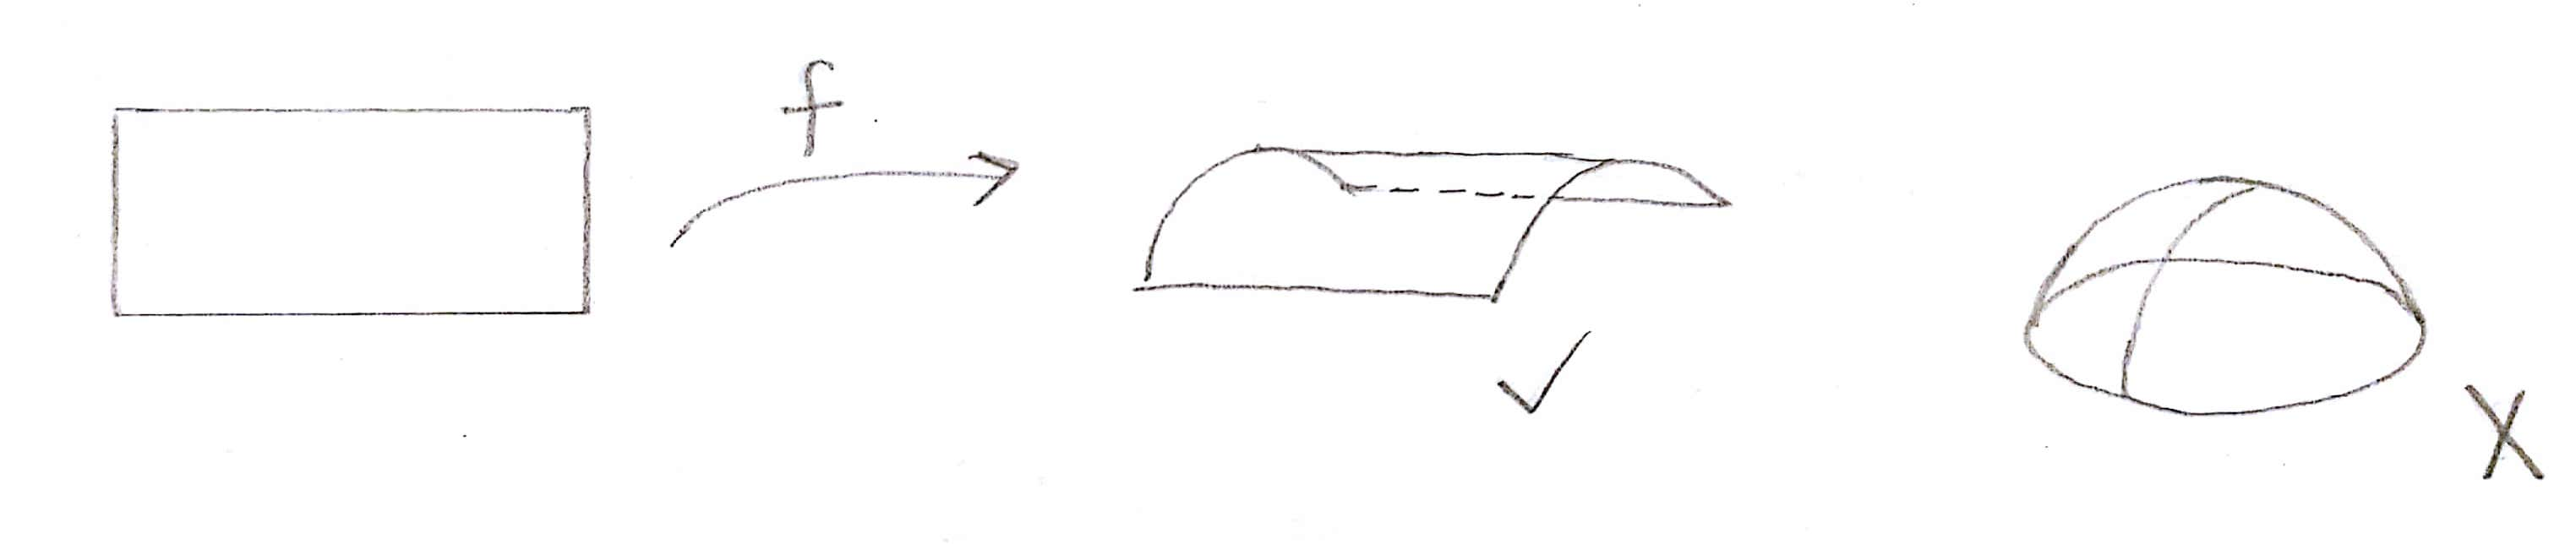
\includegraphics[width=1.0\textwidth]{chapter_7/files/isometric.jpeg}
\caption{The middle transformation has no stretch/shrink, but the rightmost transformation (a spherical cap) has stretch/shrink. }
\end{figure}
    
  \item Parametrization space should be convex. For example, if there
    is a missing/hole at the center of a manifold, an embedding will
    `fill in' the space and shorten the distance between two points
    that were originally across each other in the original manifold. 
  \end{itemize}

\end{itemize}

\subsection{LLE (Locally Linear Embedding)}
\subsubsection*{Motivation}
Isomap works well under certain conditions - but these conditions will not always hold. We need other algorithms that are capable of handling cases in which the manifold is not isometric to simple Euclidean space.

\subsubsection*{Goal}
Rather than attempting to preserve global geometry as Isomap does, we will instead find a low-dimensional embedding that preserves ``local geometry". But just what is local geometry?

\noindent \textbf{Answer}: Intuitively speaking, a manifold is some object that is locally ``flat" - if you zoom in closely enough, it looks like flat Euclidean space.

If a manifold is locally linear, then one can define ``local geometry" to be how a specific data point is linearly related to its neighbors. That is, every point in our observation set can be viewed as (approximately) a linear combination of its neighbors.

Using this particular definition of ``local geometry", we can find a low-dimensional embedding $Y$ of the given data $X$ such that the locally linear relationships between neighbors are approximately preserved - this is the LLE algorithm.

\subsubsection*{How?}
In overview - given input data $X\in \mathbb{R}^{D\times n}$, number of neighbors
$k$, embedding dimension $d$, we perform the following steps:

\begin{enumerate}
\item First we construct the $k$-NN graph (ideally, a connected graph) to find the nearest neighbors for each data point $x_i$; we denote the set of the $k$ nearest neighbors of $x_i$ as $N_i$, or $N(i)$ (but we'll prefer the latter, since the symbol $N_i$ will be used to refer to something different later).

\item Next, we find the linear representation of each data point using its neighbors with minimum discrepancy to the actual location: we take the minimum over all possible weightings of neighbors for all points

\begin{align*}
\min\limits_{W} \Phi(W) &= \sum\limits_{i=1}^n \bigg|\bigg|x_i - \sum\limits_{j\in N(i)} w_{ij} x_j\bigg|\bigg|^2\\
\text{ s.t. } & \forall i, \sum_{j} w_{ij}=1,\\
& \forall i, w_{ij}=0 \text{ for } j \not \in N(i),
\end{align*}

where $W$ is the weight matrix where entry $W_{ij} = w_{ij}$ is the weight of point $x_j$ in the linear neighbor representation of point $x_i$ (we set $w_{ij}$ to zero if $x_j$ is not a neighbor of $x_i$; and we require that the weights in the neighbor representation of any single point sum to one simply so that we may specify a unique, reasonably-scaled solution).

\item Finally, we find the low-dimensional representation that most closely fits the linear relationship of a point to its neighbors that we found in the previous step:

\begin{align*}
&\min_{Y} \Psi(Y) = \sum_{i=1}^{n} ||y_i - \sum_{j\in N(i)} w_{ij}
  y_i||^2\\ 
&\text{s.t. } Y Y^\intercal = I
\end{align*}

Here, $y_i \in \mathbb{R}^d$ is the embedding of $x_i \in \mathbb{R}^D$.
\end{enumerate}

\subsubsection*{Some notes.}
First - in step 2, why are we solving for the representation of a point by its neighbors as an optimization problem? Why not find the precise solution directly?

As it turns out, not all points \textit{can} be represented exactly as a linear combination of their neighbors. For example, in a very degenerate case, imagine we have three points sitting along a convex curve - let's call them $A, B, C$ for convenience, where $B$ lies between its neighbors $A$ and $C$. Then there's actually no way to represent $B$ as a linear combination of $A$ and $C$ - we can only represent points on the line $AC$, which cuts through the curve! (Try drawing it out if that doesn't make sense.) Another example given in class is a data point at the corner of some space. The 2D case is shown in the figure below.

Similarly, in higher-dimensional space, it's possible for all the neighbors of point $x$ to lie along (or approximately along) some subspace not containing $x$, in which case we won't be able to find an exact solution (or the ``exact" solution will involve some very large coefficients, which will effectively be just an artefact of how we happened to sample the neighbors).

\begin{figure}[H]
\centering
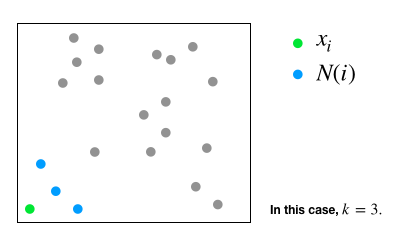
\includegraphics[width=0.5\textwidth]{chapter_7/files/no_linear_comb_case.png}
\end{figure}

The point of all these algorithms is to come up with a representation (embedding) of the data. However, this is only giving you part of the story: How are you related to your neighbors is in a linear fashion. Once this relationship is learned, now what you can do is find in a lower dimension the mapping of the data points and that respects exactly the same criteria. Now, once you have learned the relationship, find the configuration of these data points in low dimensions which respects the same relationships.

\subsection*{Details}
\subsubsection*{Step 2}
Consider the $i^\text{th}$ data point in isolation. For this single point, we'd like to minimize $\Phi (W_{i:})=||x_i-\sum_{j\in N(i)} w_{ij} x_j||^2$. So how specifically will we do this?

First let's define some notation.

\[N_i=
\begin{bmatrix}
    x_{j_1} & x_{j_2} & \dots & x_{j_k} \\
\end{bmatrix};
\]

\[w_i=
\begin{bmatrix}
    w_{ij_1} \\
    w_{ij_2} \\
    \vdots \\
    w_{ij_k} \\
\end{bmatrix}, \text{ and }
e=
\begin{bmatrix}
    1 \\
    1 \\
    \vdots \\
    1 \\
\end{bmatrix}.
\]

Note for clarity that $N_i$ is a $D \times k$ matrix, and $w_i$ and $e$ are $k \times 1$ vectors; the $j_1 \dots j_k$ in $w_i$ are the $k$ neighbors in $N(i)$.

Going back to our original minimization expression, we can rewrite the right-hand term as
\[
\sum_{j\in N(i)} w_{ij} x_j=N_i w_i.
\]

Easy enough. But what about the left-hand term?
\[
x_i = x_i e^{\intercal} w_i.
\]
``What?" you may be saying to yourself. What is this black magic? But you can verify it for yourself: because of our handy assumption that $\sum_j w_{ij} = 1$, the expression $e^\intercal w_i$ can be rewritten as
\[
e^\intercal w_i = \begin{bmatrix}
    1 & 1 & \dots & 1 \\
\end{bmatrix} w_i =
\begin{bmatrix}
    w_{ij_1} + w_{ij_2} + \dots + w_{ij_k} \\
    w_{ij_1} + w_{ij_2} + \dots + w_{ij_k} \\
    w_{ij_1} + w_{ij_2} + \dots + w_{ij_k} \\
    \text{etc.}
\end{bmatrix} =
\begin{bmatrix}
    1 \\
    1 \\
    \vdots \\
    1 \\
\end{bmatrix}.
\]

Using these rewritten terms, it follows that:
\begin{align*}
\Phi (W_{i:})
&= ||x_i e^\intercal w_i - N_i w_i||^2\\
&= ||(x_i e^\intercal-N_i)w_i||^2\\
&= w_i^\intercal (x_i e^\intercal-N_i)^\intercal (x_i e^\intercal - N_i) w_i.
\end{align*}

Now let's pause for a moment. This looks perhaps a bit complicated - but let's focus on just the middle section $(x_i e^\intercal-N_i)^\intercal (x_i e^\intercal - N_i)$. We know $x_i$ and $N_i$, and $e$ is fixed. So this entire expression in fact comes out to a known $D \times D$ matrix! Let's call it $G$. Then our optimization problem is
\begin{align*}
&\min_{w_i} w_i^\intercal G w_i \text{ where } G = (x_i e^\intercal-N_i)^\intercal (x_i e^\intercal - N_i)\\
&\text{s.t. } e^\intercal w_i = 1.
\end{align*}

(Note: at this point one might be tempted to reach for our familiar Rayleigh quotient minimization/minimum eigenvalue solution, but we can't use that here - that requires the condition $w_{i}^\intercal w_i = 1$, which we don't have.)

From here, we relax the constraint using Lagrange and take the derivative of the cost function as follows:
\begin{align*}
L(W_i,\lambda) &= W_i^\intercal G W_i - \lambda (e^\intercal W_i - 1)\\
\frac{\partial L}{\partial W_i} &= 2GW_i - \lambda e = 0\\
\Rightarrow 2GW_i &= \lambda e.
\end{align*}
If $\lambda$ is known, $w_i=G^{-1} \frac{\lambda}{2} e$. But we don't actually know $\lambda$ beforehand! Luckily, knowing $\lambda$ is not necessary: we can pick any $\lambda \neq 0$ and solve for $w_i$, and if we used something other than the true $\lambda$, this will give us a scaled version $w_{i}'$ of the true $w_i$. Recalling again that $\sum_j w_{ij} = 1$, we can normalize $w_{i}'$ to get $w_i = \dfrac{w_{i}'}{\sum_j w_{ij}'}$.

\subsubsection*{Step 3}
We consider the $i^\text{th}$ data point's embedding $y_i$. For this single point, we'd like to minimize $\Psi (y_i)=||y_i-\sum_{j\in N(i)} w_{ij} y_j||^2$.

We define the following notation:
\[Y=
\begin{bmatrix}
    y_1 & y_2 & \dots & y_n \\
\end{bmatrix}
\]
\[
W=
\begin{bmatrix}
    && && \\
    && W_{ij} && \\
    && && \\
\end{bmatrix}, \text{ where } W_{ij} = w_{ij};
\]
and $I$ is the identity matrix.

Note that here, $Y$ is a $d \times n$ matrix; both $W$ and $I$ are $n \times n$ matrices.

We use the subscript $_{:i}$ to refer to a column vector that is the $i^\text{th}$ column of a matrix. So $W_{:i}$ is the $i^\text{th}$ column of $W$, and $I_{:i}$ is the $i^\text{th}$ column of $I$.

Again we can do some rewriting:
\[
y_i = Y I_{:i}
\]
\[
\sum_{j\in N(i)} w_{ij} y_j = Y W_{:i}
\]

so for an individual point with embedding $y_i$, we can write
\[
\Psi (y_i) = ||Y I_{:i} - Y W_{:i}||^2.
\]

Summing over $i$, we can express the overall $\Psi$ term as:
\begin{align*}
\Psi(Y)
&= \sum\limits_{i=1}^n ||Y(I_{:i} - W_{:i})||^2 \\
&= ||Y (I - W)||_F^2 \\
&=\text{Tr}((I-W)^\intercal Y^\intercal Y (I-W)) \\
&=\text{Tr}(Y(I-W)(I-W)^\intercal Y^\intercal).
\end{align*}

The optimization problem becomes:
\begin{align*}
&\min_Y \text{ Tr}(YMY^\intercal) \text{ where } M = (I-W)(I-W)^\intercal \\
&\text{s.t. } Y Y^\intercal=I
\end{align*}

Observe that $Y Y^\intercal=I$ does not exactly fit the generalized eigenvalue problem formulation; we can take $Z = Y^\intercal$ so the formulation becomes:
\begin{align*}
&\min_Z \text{ Tr}(Z^\intercal MZ) \text{ where } M = (I-W)(I-W)^\intercal \\
&\text{s.t. } Z^\intercal Z=I
\end{align*}

We can solve this by taking the eigenvalue decomposition of $M$, and then takes the  $2^\text{nd},3^\text{rd},...,d+1^\text{th}$ eigenvectors.

\subsubsection*{Some observations about LLE.}
\begin{itemize}
\item It does not preserve the scale in the low-dimensional parametrization.
\item It works quite poorly in practice.
\item $(I-W)(I-W)^\intercal$ is kind of like a Laplacian of the underlying graph.
\end{itemize}

\subsection*{LE (Laplacian Eigenmaps)}
\subsubsection*{Goal}
Our goal remains the same: Find a low-dimensional representation of our high-dimensional data, which preserves local structure in the data. LLE we had the data points be related to their near neighbors in a linear fashion. The question is how do you define local structure? The answer the authors of Laplacian Eigenmaps give is a little different. They will compute some sort of similarity between data points, and once you have a notion of similarity, they will optimize for position of the low-dimensional datapoints, which will keep the same similarity. 
To summarize: Find a Low-Dimensional embedding of the original input data that preserves ``local geometry" in terms of maximally preserving similarity
between points.\\ 
\textbf{Question}: How do we measure similarity?\\
Intuitively, we want this notion of similarity to be anti-proportional to distance. In other words, we want the value of similarity to be high if the data points are a short distance apart, and we want the value of similarity to be low if the data points are far apart.\\
\textbf{Answer}: What ends up getting used is a Gaussian type function. 

\begin{definition} Similarity. \\
$w_{ij} = \txt{sim}(x_i, x_j) = \txt{exp}(-\|x_i - x_j\|^2/\sigma^2)$ where $\sigma$ is a scaling parameter. 
\end{definition}

But we're on a manifold, why are you talking about Euclidean distances and not geodesics? Well, there will be some sort of scaling parameter $\sigma$. If $\sigma$ is at the same level as a local neighbor, then locally it'll be linear anyways, so you can compute the Euclidean distance as a good approximation. Outside the neighborhood, it'll be a geodesic distance. But since it's far away, the similarity will be small. But the Euclidean distance will \textit{also} be small. Since the distance is dropping off quite sharply either way, it might be an ok approximation. $\sigma$ determines where this drop off occurs. Thus, $\sigma$ is taken at the scale of ``local neighbor''. This is a mystery in itself. There might be a paper by Larry Wasserman which could tell you. Maybe different regions of space will have different notions of locality. This is based on some notion of curvature, so the question boils down to how you can estimate the curvature of a manifold. Little work has been done, but there is some work. That's where the state of the art is. 

So now we have a notion of similarity. We want to come up with a configuration of our low-dimensional data points which will respect this similarity. So we have to come up with a cost function.\\

\subsubsection*{How?}
For Laplacian Eigenmaps, it is the following cost: 
\begin{definition} Laplacian Eigenmaps Cost Function. \\
\[
\psi(Y) := \sum_j W_{ij}\|Y_i - Y_j\|^2
\]
We want to minimize this with respect to $Y$. 
\end{definition}

If $W_{ij}$ is large, then $Y_i$ and $Y_j$ need to be close to each other. If they are dissimilar (e.g., $W_{ij} = 0$) then we don't care what happens. In this sense, the local neighborhood is preserved. What will happen in that case? Then everything gets mapped to the same thing to minimize. So you have to add a condition: We require $Y^TY = I$. 

Now, this looks like a Graph Laplacian! The cost function $\psi(Y)$ is proportional to Tr$(Y^TLY)$, where $L$ is the Graph Laplacian. In particular, it's $D - W$. $D$ is the diagonal matrix, and $W$ is the similarity matrix. Here we need to set the constraint $YY^{\top}=I$ because otherwise, we can place all points on top of each other, so that $\psi(Y)=0$.
 

\begin{itemize}
\item Define $W_{ij}=e^{-||x_i-x_j||^2}{2\sigma^2}$.
\item 
\begin{align*}
&\min_{Y} \sum_{i,j} W_{ij} ||y_i-y_j||^2\\
&\text{s.t. } Y^\intercal Y=I
\end{align*}
$\Rightarrow$
\begin{align*}
&\min_{Y} \text{tr} (Y^\intercal LY)\\
&\text{s.t. } Y^\intercal Y=I
\end{align*}
\end{itemize}
\subsubsection*{Observations}
We can compare this to LLE. This is also the Laplacian! Since we have that the row sum of the $W$ is $1$, we end up getting a $I - W$ instead of $D - W$. So the solution type is the same for both of these methods.

\subsection*{Discussion}
We can put most linear dimensionality reduction algorithms in a unified framework. Essentially, they are all special cases of Kernel-PCA. Basically, we are just changing the kernel based on the particular instantiation. 

What are we doing with PCA again? Finding a linear projection of data which is maximizing variance or minimizing distance to subspace by orthogonal projection. Kernel is saying there is a nonlinear transformation (maybe in high dimensions, maybe not) mapping $\phi$ which takes your data from the original space to another space nonlinearly. Now, we're going to do PCA in the transformed nonlinear space. 

So one way of doing it is writing down SVD. Then $X = U\Sigma V^T$, and $XX^T = U\Sigma^2 U^T$, or the eigen-decomposition of the thing. $X^TX = V\Sigma^2 V^T$. Now the interesting thing is: What will this look like? The interesting thing is that the eigenvalues of the two matrices match, but the eigenvectors don't match. But there is a relationship between them. Let us note the following: In PCA, you're taking the higher-order spectra of the data point which you want to project to. So the data would look like $U^Tx$, in PCA. If into $k$ dimensions, you take $U_k^Tx$. That is what we want to compute, but we only have the vectors $V$. But there is a relationship between them. From SVD, we have $U = XV\Sigma^{-1}$. Now if you have vectors $V$ and $\Sigma$, you can compute this. Then you get, for a new data point, $\Sigma^{-1}V^TX^Tx$. This is in terms of the inner product, which can now be generalized to kernels. So we take the kernel matrix $K = X^TX$. We can easily swap this out to our own kernel, instead of the linear inner product kernel. We just need some reasonably properties on $K$ hold true (e.g., it needs to be PSD). That is, $K(x_i, x_j) = \phi(x_i)^T\phi(x_j)$ for some nonlinear transformation $\phi$, as encoded in the matrix $K$. The punchline is that all these nonlinear dimensionality reduction techniques (IsoMap, LLE, Laplacian Eigenmaps, and others) essentially apply implicitly some sort of a nonlinearity and doing PCA. So, the only thing that changes is $K$, because the nonlinearity changes. Here we list the various cases:

\begin{itemize}
\item PCA: $K=X^\intercal X$(Linear Kernel).
\item Classical-MDS: $K=\frac{-1}{2} HD^{Euclidean}H$ where $H$ is the centering matrix. 
\item Isomap: $K=\frac{-1}{2} HD^{Geodesic}H$. For geodesic distance, we mean the shortest-path distance on the manifold.
\item LLE: In LLE, suppose we were to use $K = (I - W)(I - W)^T$. But now, we are looking at the lower order spectra, not the higher one. So we need to do some massaging to get the right kernel. Once $W$ is known (it gets learned), then essentially we compute $A = (I - W)(I - W)^T$. We need to flip the spectrum of the matrix: We could do inverse and say $K = A^{-1}$. That's option one. Another way we could do it is define $K = \lambda_{\max}I - A$. Typically, this option gets used because inverses can be bad news in terms of stability. The point is that LLE is kernel PCA with this particular kernel.  
\item Laplacian Eigenmaps (LE): $K=L^{-1}$ or $K=(\lambda_{max} I - L)$ and the result is also off in the scale of coordinate of the embedding as LLE. Also note that we can either assume the weight matrix to be known or learned.
\end{itemize}

The point is to say that all these are special cases of kernel PCA from a different kernel. So (essentially) all these nonlinear dimension reduction methods are just a matter of finding the right kernel.

There's a reason I'm telling you this story. One point is that it unifies it, but that's not the main thing. The million dollar question is: Some of these methods give you one answer, and some give you another answer. So why can you not \textit{learn} the right kernel, and see what happens. That gives rise to yet another nonlinear dimensionality reduction technique, which is called \textit{Maximum Variance Unfolding} (MVU).

\subsection*{MVU(Maximum Variance Unfolding) (aka. Semi-Definite Embedding(SDE))}

This used to be called Semidefinite Embedding (SDE). Why are we talking about this specific one? Multiple reasons. Our story began a certain way. We want to preserve local structure, this is what structure should be, here's an algorithm. Now we are not taking this recipe. What's the right way of defining local structure? MVU is by Lawrence Saul and one of his students Killian Weinberger. Around 2006, there was a lot of interest developed in terms of SDP optimization. So there were some advances made there, and machine learning people wanted to adopt those optimization techniques for machine learning problems. In terms of dimensionality reduction, you can formulate it as finding the positive semidefinite matrix itself. So there was a big rush at this time. In the early 90s, the rush was kernelizing every single method in machine learning. The mini-rush in 2006 was can we adopt the new technique of SDPs into machine learning, and this was one early incarnation where this happened in terms of nonlinear dimensionality reduction.

We're going to just formulate the problem, after it is an SDP, we just run SDP methods to get a kernel out. Then we can use kernel PCA. We need to formulate a problem to find the kernel. The question should be, what properties should hold for that particular kernel? What do you want for manifold learning? We'll list them out, and formulate it mathematically. 

\begin{enumerate}

\item Question 1: Say you want to preserve local geometry. What should hold true after applying the nonlinear transformation? How about nearest neighbors? That is, if $j \in N(i)$, we want the distances to match up: $\|\phi(x_i) - \phi(x_j)\| = \|x_i - x_j\|$. So this is one constraint. The problem is, it better be the case so that the RHS is a constant from data, and the LHS has a parameter $\phi$. It had better be the case that distances can be written as dot products. This is the key constraint!

\item What do you want for the non-neighbors to hold true? They should be far away. We'll maximize the variance subject to these kinds of constraints. This is basically doing PCA on the map. 

\end{enumerate}

Here we lay it out formally: 

\subsubsection*{Goal} Find a low-dimensional embedding of the given
data which preserves ``local geometry" in terms of finding the best
kernel.\\
Define Local Geometry in terms of distance between data points in a
local neighborhood. Denote $D\times n$ matrix
\[
X=
\begin{bmatrix}
    x_1 & x_2 & \dots & x_n \\
\end{bmatrix}
\]
and denote $d\times n$ matrix
\[
Y=
\begin{bmatrix}
    y_1 & y_2 & \dots & y_n \\
\end{bmatrix}.
\]
Want: If $j$ is a neighbor of $i$,
\begin{itemize}
\item \begin{align*}
||x_i - x_j||^2
&=||\phi (x_i)-\phi (x_j)||^2\\
&=K_{ii}+K_{jj}-2K_{ij}
\end{align*}.
\item $K$ is positive semi-definite.
\item $\sum_{ij} K_{ij}=0$.
\end{itemize}

The optimization problem can be formulated as the following:
\begin{align*}
&\max_{K} \text{tr}(K)\\
&\text{s.t. } K_{ii}+K_{jj}-2K_{ij}-||x_i-x_j||^2 \text{ if }i \text{
    and } j \text{ are neighbors}.\\ 
&\text{s.t. } \sum_{ij}K_{ij}=0\\
&\text{s.t. } K \succeq 0
\end{align*}
This is a convex optimization and can find a globally optimal solution.

\subsection*{More discussions}
Suppose we want to preserve geodesic distance approximately.
\begin{theorem}[JL-manifold]
Say n-dimensional manifold $M$ in $\mathbb{R}^D$. We know that the
volume of the manifold, Vol$(M)=V$ and global bound on curvature
$K(M)=k$. $\exists f: \mathbb{R}^D \rightarrow \mathbb{R}^d$ where
$d=O(\frac{n}{\epsilon^2}\log (Vk) )$. $\forall p,q \in M$ and
$G(p,q)$ is the geodesic path between $p,q$. Let $L(\cdot)$ be the
``length" function. $\forall p,q,n$, 
\[
1-\epsilon \leq \frac{L(G(f(p),f(q)))}{L(G(p,q))} \leq 1+\epsilon
\]
$f$ is linear (can use random projection matrix).
\end{theorem}
